\documentclass[a4paper]{article}
\usepackage{float}
\usepackage[utf8]{inputenc}
\usepackage[T1]{fontenc}
\usepackage{graphicx}
\usepackage[frenchb]{babel}
\usepackage{amsmath}
\usepackage{listings}
\usepackage{hyperref}

% define our color
\usepackage{xcolor}

% code color
\definecolor{ligthyellow}{RGB}{250,247,220}
\definecolor{darkblue}{RGB}{5,10,85}
\definecolor{ligthblue}{RGB}{1,147,128}
\definecolor{darkgreen}{RGB}{8,120,51}
\definecolor{darkred}{RGB}{160,0,0}

% other color
\definecolor{ivi}{RGB}{141,107,185}


\lstset{
    language=scilab,
    captionpos=b,
    extendedchars=true,
    frame=lines,
    numbers=left,
    numberstyle=\tiny,
    numbersep=5pt,
    keepspaces=true,
    breaklines=true,
    showspaces=false,
    showstringspaces=false,
    breakatwhitespace=false,
    stepnumber=1,
    showtabs=false,
    tabsize=3,
    basicstyle=\small\ttfamily,
    backgroundcolor=\color{ligthyellow},
    keywordstyle=\color{ligthblue},
    morekeywords={include, printf, uchar},
    identifierstyle=\color{darkblue},
    commentstyle=\color{darkgreen},
    stringstyle=\color{darkred},
}

\begin{document}

\title{VISA -- TP Couleurs}
\author{Arnaud Cojez}
\date{mercredi 9 novembre 2016}

\maketitle

\newpage
\tableofcontents
\newpage
%----------------------------------------------------------------------------------------
%	INTRODUCTION
%----------------------------------------------------------------------------------------

\section{Introduction}
Une fois la capture de la lumière maîtrisée, il nous faut définir la façon dont sera stockée l'image formée.\\
L'information des pixels d'une image peut être stockée selon différentes représentations. Par exemple, nous pouvons considérer différentes couleurs comme les composantes de l'image.\\
Ainsi, chaque opération effectuée sur une image aura un effet lié à la représentation de celle-ci.\\

Le long de ce TP, nous utiliserons l'espace de couleurs HSB (Hue-Saturation-Brightness). Celui-ci nous permet de modifier la luminance, la teinte et la saturation de l'image.\\
Les fichiers utilisés sont des images composant le test d'Ishihara, qui permet de détecter les déficiences dichromatiques telles que le daltonisme.

\begin{figure}[H]
\begin{center}
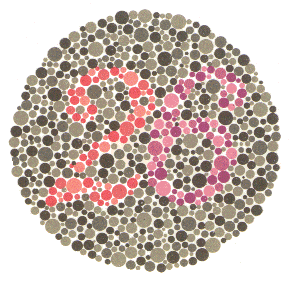
\includegraphics[width=170px]{../base/cas_1_dalton26.png}
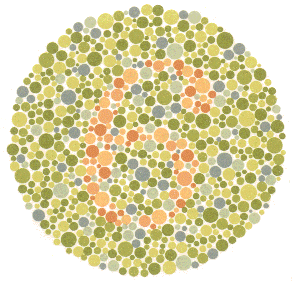
\includegraphics[width=170px]{../base/cas_4_dalton6.png}
\end{center}
\caption{Planches issues du Test d'Ishihara}
\end{figure}


\clearpage
%----------------------------------------------------------------------------------------
%	MANIPULATION DE LA LUMINANCE
%----------------------------------------------------------------------------------------

\section{Manipulation de la luminance}

\subsection{Explication}

Dans cette partie, nous possédons des images dont la luminance a été modifiée. Nous verrons donc des images tirant plus vers le blanc ou vers le noir.\\
Le but est de comparer l'image originale et l'image modifiée en utilisant un espace de couleur approprié.\\
Il nous faudra par conséquent mettre en évidence les différences, faire une estimation des retouches à apporter pour retrouver l'image originale, et enfin retoucher cette image, en analysant le résultat obtenu.

\subsubsection{Cas 1}

\begin{figure}[H]
\begin{center}
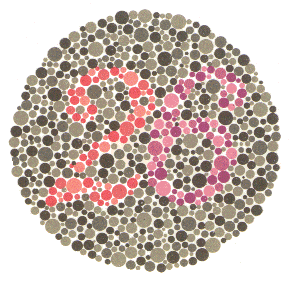
\includegraphics[width=170px]{../base/cas_1_dalton26.png}
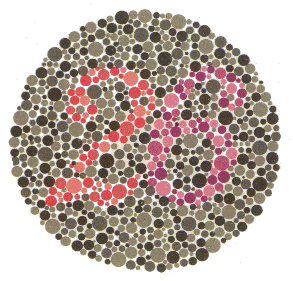
\includegraphics[width=170px]{../base/cas_1_luminance.png}
\end{center}
\caption{À gauche, image originale. À droite, image modifiée}
\end{figure}

\begin{figure}[H]
\begin{center}
\includegraphics[width=170px]{../resultats/e1_q1_k1_26.png}
\includegraphics[width=170px]{../resultats/e1_q1_k1_lumi.png}
\end{center}
\caption{Visualisation des 2 images dans l'espace HSB}
\end{figure}

Nous constatons en analysant la répartition des couleurs dans l'espace HSB que la luminance de l'image modifiée à été diminuée.\\
Après une augmentation de la luminance de 20 dans le Color Inspector 3D, nous constatons que l'image est relativement similaire à l'image d'origine.

\subsubsection{Cas 2}

\begin{figure}[H]
\begin{center}
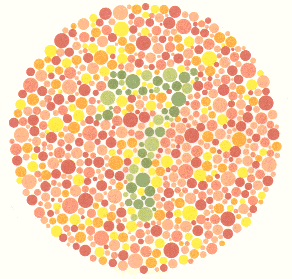
\includegraphics[width=170px]{../base/cas_2_dalton7.png}
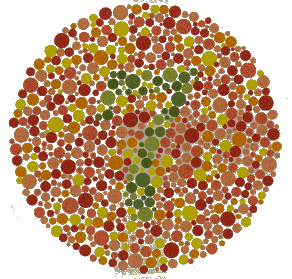
\includegraphics[width=170px]{../base/cas_2_luminance.png}
\end{center}
\caption{À gauche, image originale. À droite, image modifiée}
\end{figure}

\begin{figure}[H]
\begin{center}
\includegraphics[width=170px]{../resultats/e1_q1_k2_7.png}
\includegraphics[width=170px]{../resultats/e1_q1_k2_lumi.png}
\end{center}
\caption{Visualisation des 2 images dans l'espace HSB}
\end{figure}

Nous constatons que la luminance de l'image modifiée à également été diminuée, de façon plus importante.\\
Après une augmentation de la luminance de 80, nous retrouvons plus ou moins l'image de base.

\subsubsection{Cas 3}

\begin{figure}[H]
\begin{center}
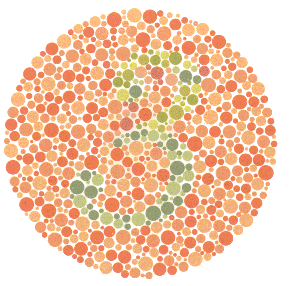
\includegraphics[width=170px]{../base/cas_3_dalton3.png}
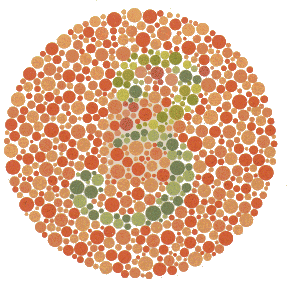
\includegraphics[width=170px]{../base/cas_3_luminance.png}
\end{center}
\caption{À gauche, image originale. À droite, image modifiée}
\end{figure}

\begin{figure}[H]
\begin{center}
\includegraphics[width=170px]{../resultats/e1_q1_k3_3.png}
\includegraphics[width=170px]{../resultats/e1_q1_k3_lumi.png}
\end{center}
\caption{Visualisation des 2 images dans l'espace HSB}
\end{figure}

Nous constatons qu'ici aussi la luminance a été diminuée, mais la différence semble moins importante.\\
Après une augmentation de la luminance de 30, nous retrouvons plus ou moins l'image de base.

\subsubsection{Cas 4}

\begin{figure}[H]
\begin{center}
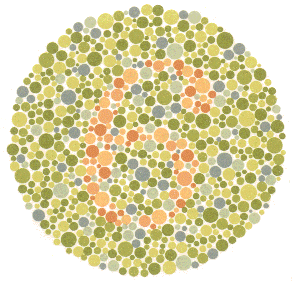
\includegraphics[width=170px]{../base/cas_4_dalton6.png}
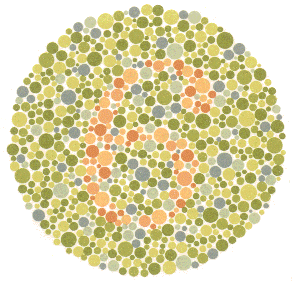
\includegraphics[width=170px]{../base/cas_4_luminance.png}
\end{center}
\caption{À gauche, image originale. À droite, image modifiée}
\end{figure}

\begin{figure}[H]
\begin{center}
\includegraphics[width=170px]{../resultats/e1_q1_k4_6.png}
\includegraphics[width=170px]{../resultats/e1_q1_k4_lumi.png}
\end{center}
\caption{Visualisation des 2 images dans l'espace HSB}
\end{figure}

Ici nous pouvons constater que l'image n'a pas été modifiée.

\subsection{Résultats}

Nous avons implémenté une macro ImageJ (disponible en annexe) permettant d'additionner une valeur donnée aux 3 canaux RGB de l'image.\\
Cette opération a pour effet d'augmenter la luminance de l'image.\\

Par conséquent, nous avons pu tester les valeurs estimées dans la partie précédente et constater si les résultats correspondent réellement aux images initiales.

\subsubsection{Cas 1}
Nous avons utilisé la macro sur l'image modifiée, en lui donnant la valeur estimée 20.

\begin{figure}[H]
\begin{center}
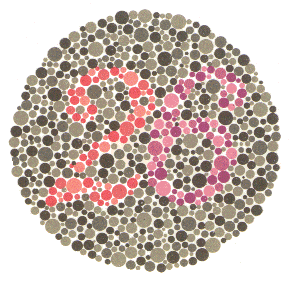
\includegraphics[width=170px]{../base/cas_1_dalton26.png}
\includegraphics[width=170px]{../resultats/e1_q2_k1_luminance.png}
\end{center}
\caption{À gauche, image originale. À droite, image retouchée}
\end{figure}

Nous constatons que l'image est identique en tous points à la première, ce qui confirme nos estimations.\\
En effet, nous pouvons voir ci-dessous que la carte des différences entre les 2 images est totalement noire.\\
De plus, l'histogramme associé à cette carte des différences nous indique que la valeur maximale et la moyenne des pixels sont à 0, ce qui prouve l'absence de différences entre les deux images.

\begin{figure}[H]
\begin{center}
\includegraphics[width=170px]{../resultats/e1_q2_k1_diff.png}
\includegraphics[width=170px]{../resultats/e1_q2_k1_diff_hist.png}
\end{center}
\caption{Carte des différences et son histogramme}
\end{figure}

\clearpage
\subsubsection{Cas 2}
Nous avons utilisé la macro sur l'image modifiée, en lui donnant la valeur estimée 80.

\begin{figure}[H]
\begin{center}
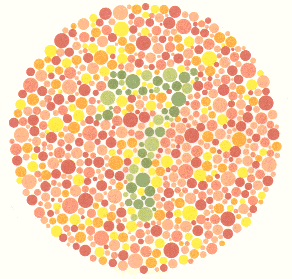
\includegraphics[width=170px]{../base/cas_2_dalton7.png}
\includegraphics[width=170px]{../resultats/e1_q2_k2_luminance.png}
\end{center}
\caption{À gauche, image originale. À droite, image retouchée}
\end{figure}

Nous constatons que l'image est quasiment identique à l'image de base. Cependant, il existe certaines différences entre les deux.\\
En effet, bien que la carte des différences semble totalement noire, avec l'histogramme nous pouvons constater que quelques pixels sont légérement différents (moyenne de 1.348 et maximum de 8).

\begin{figure}[H]
\begin{center}
\includegraphics[width=170px]{../resultats/e1_q2_k2_diff.png}
\includegraphics[width=170px]{../resultats/e1_q2_k2_diff_hist.png}
\end{center}
\caption{Carte des différences et son histogramme}
\end{figure}

\clearpage
\subsubsection{Cas 3}
Nous avons utilisé la macro sur l'image modifiée, en lui donnant la valeur estimée 30.

\begin{figure}[H]
\begin{center}
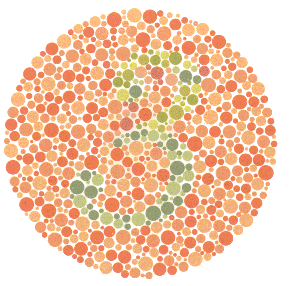
\includegraphics[width=170px]{../base/cas_3_dalton3.png}
\includegraphics[width=170px]{../resultats/e1_q2_k3_luminance.png}
\end{center}
\caption{À gauche, image originale. À droite, image retouchée}
\end{figure}

Nous constatons que l'image est de nouveau identique à l'image de base. Ce qui confirme l'estimation faite plus tôt.

\begin{figure}[H]
\begin{center}
\includegraphics[width=170px]{../resultats/e1_q2_k3_diff.png}
\includegraphics[width=170px]{../resultats/e1_q2_k3_diff_hist.png}
\end{center}
\caption{Carte des différences et son histogramme}
\end{figure}

\subsubsection{Cas 4}
Il n'y avait ici aucune modification à faire.

\clearpage
%----------------------------------------------------------------------------------------
% RÉTABLISSEMENT DE LA SATURATION
%----------------------------------------------------------------------------------------

\section{Rétablissement de la saturation}

\subsection{Explication}

Ici nous sommes en présence d'images dont la saturation a été modifiée. Les couleurs seront donc plus ou moins vives en fonction des modifications effectuées.\\
Nous estimerons de quel facteur la saturation aura été modifiée et nous analyserons nos résultats.\\
{\em (Les cas sont traités dans l'ordre des questions du TP, le cas 2 est donc traité avant le cas 1.)}

\subsubsection{Cas 2}

\begin{figure}[H]
\begin{center}
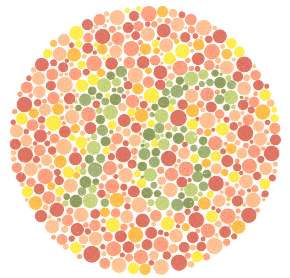
\includegraphics[width=170px]{../base/cas_2_dalton16.png}
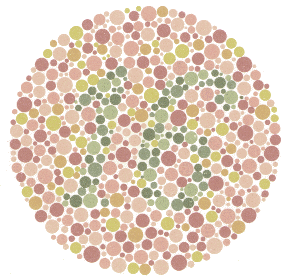
\includegraphics[width=170px]{../base/cas_2_dalton16-question2-1.png}
\end{center}
\caption{Visualisation des 2 images dans l'espace HSB}
\end{figure}

\begin{figure}[H]
\begin{center}
\includegraphics[width=170px]{../resultats/e2_q1_k2_16.png}
\includegraphics[width=170px]{../resultats/e2_q1_k2_modif.png}
\end{center}
\caption{Visualisation des 2 images dans l'espace HSB}
\end{figure}

Nous constatons ici que les couleurs sont plus fades, nous pouvons donc en conclure que la saturation a été diminuée.\\
Après quelques manipulations dans le plugin Color Inspector 3D, nous pensons qu'il faut multiplier la saturation par 2 afin de retrouver l'image de base.

\subsubsection{Cas 1}

\begin{figure}[H]
\begin{center}
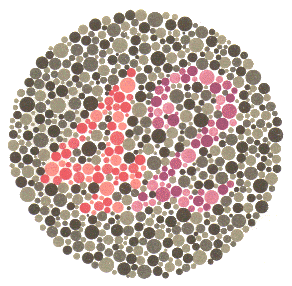
\includegraphics[width=170px]{../base/cas_1_dalton42.png}
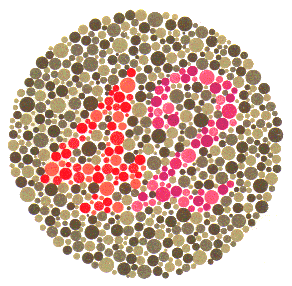
\includegraphics[width=170px]{../base/cas_1_dalton42-question2-2.png}
\end{center}
\caption{Visualisation des 2 images dans l'espace HSB}
\end{figure}

\begin{figure}[H]
\begin{center}
\includegraphics[width=170px]{../resultats/e2_q2_k1_42.png}
\includegraphics[width=170px]{../resultats/e2_q2_k1_modif.png}
\end{center}
\caption{Visualisation des 2 images dans l'espace HSB}
\end{figure}

Nous constatons ici que les couleurs sont plus vives, nous pouvons donc en conclure que la saturation a été augmentée.\\
Après quelques manipulations, nous estimons qu'il faut multiplier la saturation par 0.5 afin de retrouver l'image de base.

\clearpage
\subsection{Résultats}
Nous avons implémenté une macro ImageJ (disponible en annexe) permettant de multiplier le canal S (Saturation) d'une image par un facteur donné.\\

Par conséquent, nous avons pu tester les valeurs estimées dans la partie précédente et constater si les résultats correspondent réellement aux images initiales.

\subsubsection{Cas 2}
Nous avons utilisé la macro sur l'image modifiée, en lui donnant le facteur estimé 2.

\begin{figure}[H]
\begin{center}
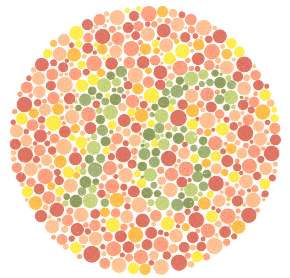
\includegraphics[width=170px]{../base/cas_2_dalton16.png}
\includegraphics[width=170px]{../resultats/e2_q3_1_modif.png}
\end{center}
\caption{À gauche, image originale. À droite, image retouchée}
\end{figure}

Nous constatons que l'image s'approche de l'image de base, mais il subsiste beaucoup de différences, liées à la luminance de l'image.

\begin{figure}[H]
\begin{center}
\includegraphics[width=170px]{../resultats/e2_q3_1_diff.png}
\includegraphics[width=170px]{../resultats/e2_q3_1_diff_hist.png}
\end{center}
\caption{Carte des différences et son histogramme}
\end{figure}

\clearpage
\subsubsection{Cas 1}
Nous avons utilisé la macro sur l'image modifiée, en lui donnant le facteur estimé 0.5.

\begin{figure}[H]
\begin{center}
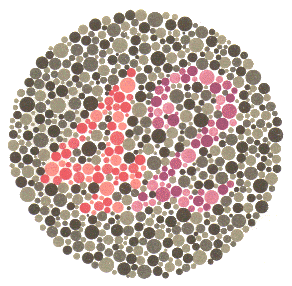
\includegraphics[width=170px]{../base/cas_1_dalton42.png}
\includegraphics[width=170px]{../resultats/e2_q3_2_modif.png}
\end{center}
\caption{À gauche, image originale. À droite, image retouchée}
\end{figure}

Nous constatons que l'image s'approche de l'image de base, mais il subsiste ici aussi beaucoup de différences entre les deux.\\
Nous pensons que ces différences sont liées à la luminance de l'image.

\begin{figure}[H]
\begin{center}
\includegraphics[width=170px]{../resultats/e2_q3_2_diff.png}
\includegraphics[width=170px]{../resultats/e2_q3_2_diff_hist.png}
\end{center}
\caption{Carte des différences et son histogramme}
\end{figure}

\clearpage
%----------------------------------------------------------------------------------------
%	TRANSFORMATION DE LA TEINTE
%----------------------------------------------------------------------------------------

\section{Transformation de la teinte}

\subsection{Explication}

Dans ce cas nous avons une image dont la teinte a été modifiée. Les couleurs auront la même intensité, mais auront des valeurs et teintes différentes.\\
Nous pouvons représenter l'ensemble des teintes par un cercle contenant toutes les couleurs.

\begin{figure}[H]
\begin{center}
\includegraphics[width=140px]{RGB_color_wheel_360.png}
\end{center}
\caption{Cercle Chromatique (Source : \href{https://commons.wikimedia.org/wiki/File:RGB_color_wheel_360.svg}{Wikipédia})}
\end{figure}

Par conséquent, nous modifierons la teinte en faisant des rotations autour de ce cercle. Nous utiliserons donc comme unité les degrés. Il faudra ensuite convertir ces degrés en valeurs numériques ($rot * \frac{256}{360}$).\\

Nous estimerons de quel degré la teinte devra être modifiée et nous analyserons nos résultats par la suite.\\

\subsubsection{Cas 3}

\begin{figure}[H]
\begin{center}
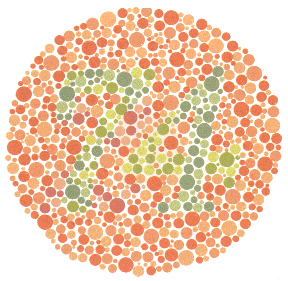
\includegraphics[width=170px]{../base/cas_3_dalton74.png}
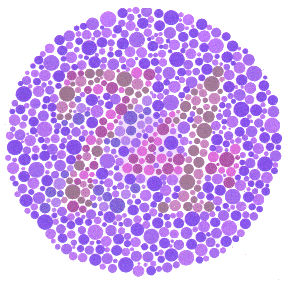
\includegraphics[width=170px]{../base/cas_3_dalton74_question3_1.png}
\end{center}
\caption{À gauche, image originale. À droite, image modifiée}
\end{figure}

\begin{figure}[H]
\begin{center}
\includegraphics[width=170px]{../resultats/e3_q1_diff.png}
\includegraphics[width=170px]{../resultats/e3_q1_diff_hist.png}
\end{center}
\caption{Visualisation des 2 images dans l'espace HSB}
\end{figure}

Les couleurs ici sont totalement différentes, il nous faut donc manipuler la teinte à l'aide du plugin Color Inspector 3D.\\
Nous retrouvons à peu près la même image avec une rotation de 120${^\circ}$ (ou -240${^\circ}$).

\subsection{Résultats}
Nous avons implémenté une macro ImageJ (disponible en annexe) permettant de faire une rotation de la teinte d'une image avec un angle donné. Pour ce faire, nous convertissons l'angle sur l'échelle d'un octet (de 360 à 256) à l'aide de cette opération : $rot * \frac{256}{360}$ puis additionnons le résultat à la teinte courante.\\

Nous pouvons désormais tester les valeurs estimées dans la partie précédente et constater si les résultats correspondent réellement à l'image initiale.

\subsubsection{Cas 3}

\begin{figure}[H]
\begin{center}
\includegraphics[width=170px]{../base/cas_3_dalton74.png}
\includegraphics[width=170px]{../resultats/e3_q1_modif.png}
\end{center}
\caption{À gauche, image originale. À droite, image retouchée}
\end{figure}

Pour une valeur de 120${^\circ}$, la couleur de fond est correcte mais pas celle du 74. (Il faut probablement utiliser un modulo pour la rotation. En effet, nous avons directement utilisé la fonction 'Add...' de ImageJ)\\

Nous effectuons donc une rotation de -240${^\circ}$, ce qui nous donne des résultats s'approchant fortement de l'image de base.

\begin{figure}[H]
\begin{center}
\includegraphics[width=170px]{../resultats/e3_q1_diff.png}
\includegraphics[width=170px]{../resultats/e3_q1_diff_hist.png}
\end{center}
\caption{Carte des différences et son histogramme}
\end{figure}

\clearpage

%----------------------------------------------------------------------------------------
%	ANALYSE DANS DES ESPACES COULEURS ADAPTÉS
%----------------------------------------------------------------------------------------

\section{Analyse dans des espaces couleur adaptés}

\subsection{Explication}

Pour cette partie, il nous fallait comparer les deux images ci-dessous.

\begin{figure}[H]
\begin{center}
\includegraphics[width=170px]{../base/cas_3_dalton74.png}
\includegraphics[width=170px]{../base/cas3_dalton74_question4_1.png}
\end{center}
\caption{À gauche, image originale. À droite, image modifiée}
\end{figure}

\begin{figure}[H]
\begin{center}
\includegraphics[width=170px]{../resultats/e4_visu_original.png}
\includegraphics[width=170px]{../resultats/e4_visu_modif.png}
\end{center}
\caption{Visualisation des 2 images dans l'espace HSB}
\end{figure}

\clearpage
\subsection{Analyse}

Nous constatons que dans la deuxième image, tous les pixels ont la même teinte (voir fig. 29).
En observant attentivement la deuxième image, nous pouvons voir se réveler un 21 (pixels moins saturés) ainsi que le 74 de l'image originale (pixels plus clairs).

Cela se voit mieux lorsque nous utilisons l'espace de couleurs KLT/PCA.

\begin{figure}[H]
\begin{center}
\includegraphics[width=170px]{../resultats/e4_21_74.png}
\includegraphics[width=170px]{../resultats/e4_21_74_visu.png}
\end{center}
\caption{Visualisation des 2 images dans l'espace KLT/PCA}
\end{figure}

Ici nous pouvons voir plus clairement le 21 (points gris), et le 74 (composé des points gris et jaune clairs).

\clearpage
%----------------------------------------------------------------------------------------
%	MODIFICATION DE LA LUMINANCE ADAPTÉE
%----------------------------------------------------------------------------------------

\section{Modification de la luminance adaptée}

\subsection{Explication}

Le but de cette partie est de retrouver la différence entre les deux images suivantes.

\begin{figure}[H]
\begin{center}
\includegraphics[width=170px]{../base/cas_1_dalton42.png}
\includegraphics[width=170px]{../base/cas_1_dalton42-question5.png}
\end{center}
\caption{À gauche, image originale. À droite, image modifiée}
\end{figure}

\begin{figure}[H]
\begin{center}
\includegraphics[width=170px]{../resultats/e5_visu_original.png}
\includegraphics[width=170px]{../resultats/e5_visu_modif.png}
\end{center}
\caption{Visualisation des 2 images dans l'espace HSB}
\end{figure}

\clearpage
\subsection{Analyse}

Nous constatons que les pixels ont la même teinte et saturation.\\
La différence se situe au niveau de la luminance. En effet, si le pixel est situé en-dessous d'un certain seuil de luminance, on augmentera la luminance de celui-ci.

\clearpage
%----------------------------------------------------------------------------------------

%----------------------------------------------------------------------------------------
%	CONCLUSION
%----------------------------------------------------------------------------------------

\section{Conclusion}
Nous avons pu constater qu'une image possède plusieurs composantes, mais que celles-ci peuvent différer en fonction de la représentation de l'image, ou espace colorimétrique.\\

Chaque opération sur un espace colorimétrique aura un effet propre à l'espace. De plus, les jeux de composantes pourront mettre en évidence différents phénomènes apparaissant sur l'image.\\
Il existe cependant une limite aux opérations sur les espaces colorimétriques. Lorsqu'une image a été modifiée, il est possible de perdre de l'information à cause d'un effet de plancher/plafond.\\

Il peut donc être utile de convertir un espace colorimétrique en un autre afin de pouvoir profiter d'opérations spécifiques, ou pour analyser la composition de l'image sous un autre angle.

\clearpage
%----------------------------------------------------------------------------------------

\section{Annexe}

\subsection{Manipulation de la luminance}
\lstinputlisting{../add_brightness.ijm}

\subsection{Rétablissement de la saturation}
\lstinputlisting{../mul_saturation.ijm}

\subsection{Transformation de la teinte}
\lstinputlisting{../change_hue.ijm}

\end{document}
